\section{Spontaneous Emission and the End of the Universe}

\subsection{Introduction to the Cosmic Excited State}
In the preceding chapters, we established the paradigm of Excited-State Cosmology, wherein the observable universe is modeled as the internal manifold of an excited hyper-electron. A natural consequence of any bound quantum system in an excited state is its eventual decay to a lower energy configuration via the emission of a gauge boson. In the context of our cosmic framework, this implies that the asymptotic future of the universe is not the asymptotically slow thermodynamic equilibrium known as the Heat Death, but rather a sudden, discontinuous quantum jump. This transition, analogous to spontaneous emission in atomic physics, would manifest as an instantaneous cosmic collapse accompanied by the emission of a hyper-photon. \cite{Zwicky1933, Starobinsky1980, Smoot1992}

In this chapter, we derive the transition rate for this catastrophic cosmic event. We will build upon the fundamental principles of quantum electrodynamics (QED), adapting the derivations of the Einstein A-coefficient and electric dipole transition moments to the hyper-dimensional parameters of our cosmological model. The profound consequence of this derivation is that the end of time is not a gradual fading into cold darkness, but a spontaneous, indeterministic collapse dictated by the laws of quantum probability.

\subsection{Quantization of the Hyper-Electromagnetic Field}
To describe spontaneous emission, one cannot rely on semi-classical radiation theory; instead, we must quantize the hyper-electromagnetic field residing in the bulk space encompassing our universe. The vacuum state of this hyper-photon field, $|0\rangle$, possesses non-zero zero-point energy fluctuations. It is precisely these vacuum fluctuations that perturb the excited hyper-electron, inducing the spontaneous transition.

We begin with the classical hyper-electromagnetic vector potential $\vec{A}(\vec{r}, t)$ in the Coulomb gauge, where $\nabla \cdot \vec{A} = 0$. Promoting this field to a quantum mechanical operator, we expand it in a complete set of transverse plane waves:
\begin{equation}
    \hat{\vec{A}}(\vec{r}, t) = \sum_{\vec{k}, \lambda} \sqrt{\frac{\hbar}{2 \epsilon_0 \omega_k V}} \left[ \hat{a}_{\vec{k}, \lambda} \vec{\epsilon}_{\vec{k}, \lambda} e^{i(\vec{k} \cdot \vec{r} - \omega_k t)} + \hat{a}_{\vec{k}, \lambda}^\dagger \vec{\epsilon}_{\vec{k}, \lambda}^* e^{-i(\vec{k} \cdot \vec{r} - \omega_k t)} \right]
\end{equation}
Here, $\vec{k}$ represents the wave vector of the mode, $\lambda \in \{1, 2\}$ indexes the two independent transverse polarization states, $\vec{\epsilon}_{\vec{k}, \lambda}$ is the polarization unit vector satisfying $\vec{k} \cdot \vec{\epsilon}_{\vec{k}, \lambda} = 0$, and $\omega_k = c|\vec{k}|$ is the angular frequency. The parameter $V$ denotes the quantization volume within the hyper-bulk. The operators $\hat{a}_{\vec{k}, \lambda}$ and $\hat{a}_{\vec{k}, \lambda}^\dagger$ are the hyper-photon annihilation and creation operators, respectively. They obey the standard bosonic commutation relations:
\begin{equation}
    [\hat{a}_{\vec{k}, \lambda}, \hat{a}_{\vec{k}', \lambda'}^\dagger] = \delta_{\vec{k}, \vec{k}'} \delta_{\lambda, \lambda'} \quad \text{and} \quad [\hat{a}_{\vec{k}, \lambda}, \hat{a}_{\vec{k}', \lambda'}] = [\hat{a}_{\vec{k}, \lambda}^\dagger, \hat{a}_{\vec{k}', \lambda'}^\dagger] = 0
\end{equation}
The Hamiltonian of the free hyper-electromagnetic field can thus be expressed as the sum over all decoupled harmonic oscillators:
\begin{equation}
    \hat{H}_{rad} = \sum_{\vec{k}, \lambda} \hbar \omega_k \left( \hat{a}_{\vec{k}, \lambda}^\dagger \hat{a}_{\vec{k}, \lambda} + \frac{1}{2} \right)
\end{equation}
The term $\frac{1}{2}\hbar\omega_k$ represents the critical vacuum energy responsible for spontaneous emission.

\subsection{The Interaction Hamiltonian and Dipole Approximation}
The interaction between the hyper-electron and the quantized hyper-electromagnetic field is governed by the principle of minimal coupling. The canonical momentum $\hat{\vec{p}}$ of the hyper-electron is replaced by $\hat{\vec{p}} - q\hat{\vec{A}}$, leading to the kinetic energy operator $\frac{1}{2m}(\hat{\vec{p}} - q\hat{\vec{A}})^2$. Expanding this expression yields the unperturbed kinetic energy $\frac{\hat{p}^2}{2m}$ and interaction terms. To first order in the field, the dominant interaction Hamiltonian is:
\begin{equation}
    \hat{H}_{int} = -\frac{q}{m} \hat{\vec{p}} \cdot \hat{\vec{A}}
\end{equation}
In deriving the Einstein A-coefficient, we invoke the electric dipole approximation. The characteristic wavelength $\lambda_{rad}$ of the emitted hyper-photon is presumed to be orders of magnitude larger than the spatial extent $a_0$ of the hyper-electron's internal manifold (our universe), i.e., $ka_0 \ll 1$. Under this condition, the spatial phase factor $e^{i\vec{k} \cdot \vec{r}}$ in the vector potential is approximately unity.

By utilizing the canonical commutation relation $[\hat{\vec{r}}, \hat{H}_0] = \frac{i\hbar}{m} \hat{\vec{p}}$, where $\hat{H}_0$ is the unperturbed hyper-electron Hamiltonian, we can perform a gauge transformation (the G\"oppert-Mayer transformation) to rewrite the interaction Hamiltonian in the more intuitive length gauge:
\begin{equation}
    \hat{H}_{int} = - \hat{\vec{d}} \cdot \hat{\vec{E}}
\end{equation}
where $\hat{\vec{d}} = q \hat{\vec{r}}$ defines the electric dipole moment operator of the hyper-electron. The electric field operator $\hat{\vec{E}}$, evaluated at the position of the hyper-electron (taken as the origin $\vec{r}=0$), is given by $-\frac{\partial \hat{\vec{A}}}{\partial t}$:
\begin{equation}
    \hat{\vec{E}}(0, t) = i \sum_{\vec{k}, \lambda} \sqrt{\frac{\hbar \omega_k}{2 \epsilon_0 V}} \vec{\epsilon}_{\vec{k}, \lambda} \left[ \hat{a}_{\vec{k}, \lambda} e^{-i\omega_k t} - \hat{a}_{\vec{k}, \lambda}^\dagger e^{i\omega_k t} \right]
\end{equation}

\subsection{Transition Matrix Element and Fermi's Golden Rule}
Let us define the initial state of the coupled system as $|i\rangle = |\psi_{exc}\rangle \otimes |0\rangle$. Here, $|\psi_{exc}\rangle$ represents the hyper-electron in its excited cosmic state---the state corresponding to our presently expanding universe---and $|0\rangle$ denotes the hyper-photon vacuum. The final state, subsequent to spontaneous emission, is $|f\rangle = |\psi_{gr}\rangle \otimes |1_{\vec{k}, \lambda}\rangle$, indicating that the hyper-electron has collapsed into its ground state $|\psi_{gr}\rangle$, and a single hyper-photon with momentum $\hbar\vec{k}$ and polarization $\lambda$ has been emitted into the bulk.

The transition probability per unit time from $|i\rangle$ to the continuum of final states $|f\rangle$ is provided by first-order time-dependent perturbation theory, yielding Fermi's Golden Rule:
\begin{equation}
    \Gamma_{i \to f} = \frac{2\pi}{\hbar} |\langle f | \hat{H}_{int} | i \rangle|^2 \delta(E_f - E_i)
\end{equation}
The total initial energy is $E_i = E_{exc}$, while the total final energy is $E_f = E_{gr} + \hbar \omega_k$. Thus, the Dirac delta function enforces exact energy conservation: $\hbar \omega_k = E_{exc} - E_{gr} \equiv \hbar \omega_{0}$, dictating that the emitted hyper-photon possesses an angular frequency $\omega_0$ corresponding to the energy gap.

We now evaluate the transition matrix element. Substituting the length-gauge interaction Hamiltonian and the electric field operator, we focus on the creation operator $\hat{a}_{\vec{k}, \lambda}^\dagger$ since the annihilation operator annihilates the initial vacuum state:
\begin{align}
    \langle f | \hat{H}_{int} | i \rangle &= - \langle \psi_{gr} | \otimes \langle 1_{\vec{k}, \lambda} | \left( \hat{\vec{d}} \cdot \hat{\vec{E}} \right) |\psi_{exc}\rangle \otimes |0\rangle \nonumber \\
    &= i \sqrt{\frac{\hbar \omega_k}{2 \epsilon_0 V}} \langle \psi_{gr} | \hat{\vec{d}} | \psi_{exc} \rangle \cdot \vec{\epsilon}_{\vec{k}, \lambda}^* \langle 1_{\vec{k}, \lambda} | \hat{a}_{\vec{k}, \lambda}^\dagger | 0 \rangle \nonumber \\
    &= i \sqrt{\frac{\hbar \omega_k}{2 \epsilon_0 V}} \left( \vec{d}_{gr, exc} \cdot \vec{\epsilon}_{\vec{k}, \lambda}^* \right)
\end{align}
where we define the transition dipole moment $\vec{d}_{gr, exc} = \langle \psi_{gr} | \hat{\vec{d}} | \psi_{exc} \rangle$. This vector quantity determines the intrinsic strength of the coupling between the cosmic excited state and the ground state vacuum.

\subsection{Density of States and Integration}
To ascertain the total spontaneous emission rate, representing the macroscopic Einstein $A$-coefficient, we must integrate the differential transition rate over all possible final states of the hyper-photon. This involves summing over the discrete polarization states $\lambda$ and integrating over the continuous distribution of wave vectors $\vec{k}$.

In the limit of a macroscopically large quantization volume $V$, the sum over discrete modes $\vec{k}$ transitions into an integral over momentum space:
\begin{equation}
    \sum_{\vec{k}} \longrightarrow \frac{V}{(2\pi)^3} \int d^3k = \frac{V}{(2\pi)^3} \int_0^\infty k^2 dk \int d\Omega
\end{equation}
where $d\Omega = \sin\theta d\theta d\phi$ is the differential solid angle. Applying the linear dispersion relation for massless hyper-photons, $\omega_k = ck$, we substitute $k = \omega_k / c$ and $dk = d\omega_k / c$. The density of states, expressing the number of phase space states per unit energy interval $dE = \hbar d\omega_k$, becomes:
\begin{equation}
    \rho(E) dE = \rho(\omega_k) d(\hbar \omega_k) = \frac{V \omega_k^2}{(2\pi c)^3 \hbar} d(\hbar \omega_k) d\Omega
\end{equation}
This quantifies the density of available vacuum modes that can stimulate the transition.

\subsection{Derivation of the Einstein A-Coefficient~\cite{Einstein1916Rad}}
The total decay rate $A$ is the integral of the differential rate over all solid angles and energies:
\begin{equation}
    A = \int d\Omega \int d(\hbar \omega_k) \sum_{\lambda=1,2} \frac{2\pi}{\hbar} \left( \frac{\hbar \omega_k}{2 \epsilon_0 V} \right) |\vec{d}_{gr, exc} \cdot \vec{\epsilon}_{\vec{k}, \lambda}^*|^2 \frac{V \omega_k^2}{(2\pi c)^3 \hbar} \delta(\hbar \omega_k - \hbar \omega_0)
\end{equation}
The integration over $d(\hbar \omega_k)$ is trivially executed by virtue of the Dirac delta function, which enforces $\omega_k = \omega_0$:
\begin{equation}
    A = \frac{\omega_0^3}{8 \pi^2 \epsilon_0 \hbar c^3} \int d\Omega \sum_{\lambda=1,2} |\vec{d}_{gr, exc} \cdot \vec{\epsilon}_{\vec{k}, \lambda}^*|^2
\end{equation}
To perform the angular integration, we must evaluate the polarization sum. The two transverse polarization vectors $\vec{\epsilon}_{\vec{k}, 1}$ and $\vec{\epsilon}_{\vec{k}, 2}$, along with the propagation direction $\hat{k} = \vec{k}/|\vec{k}|$, form an orthonormal triad. Thus, by completeness:
\begin{equation}
    \sum_{\lambda=1,2} (\vec{d}_{gr, exc} \cdot \vec{\epsilon}_{\vec{k}, \lambda}^*)(\vec{d}_{gr, exc} \cdot \vec{\epsilon}_{\vec{k}, \lambda}) = |\vec{d}_{gr, exc}|^2 - |\vec{d}_{gr, exc} \cdot \hat{k}|^2
\end{equation}
Without loss of generality, let us orient our coordinate system such that the transition dipole moment $\vec{d}_{gr, exc}$ defines the polar $z$-axis. The dot product with the unit vector $\hat{k}$ is then simply $|\vec{d}_{gr, exc}|\cos\theta$, where $\theta$ is the polar angle between $\vec{k}$ and $\vec{d}_{gr, exc}$. The polarization sum reduces to:
\begin{equation}
    \sum_{\lambda=1,2} |\vec{d}_{gr, exc} \cdot \vec{\epsilon}_{\vec{k}, \lambda}^*|^2 = |\vec{d}_{gr, exc}|^2 (1 - \cos^2\theta) = |\vec{d}_{gr, exc}|^2 \sin^2\theta
\end{equation}
We now perform the integration over the full solid angle $d\Omega$:
\begin{align}
    \int d\Omega \sin^2\theta &= \int_0^{2\pi} d\phi \int_0^\pi d\theta \sin\theta (\sin^2\theta) \nonumber \\
    &= 2\pi \int_{-1}^1 (1 - x^2) dx \quad \text{(where } x = \cos\theta \text{)} \nonumber \\
    &= 2\pi \left[ x - \frac{x^3}{3} \right]_{-1}^1 = 2\pi \left( \frac{4}{3} \right) = \frac{8\pi}{3}
\end{align}
Substituting this geometrical factor back into our expression for the total decay rate, we arrive at the definitive Einstein $A$-coefficient for the hyper-electron universe:
\begin{equation}
    A = \frac{\omega_0^3 |\vec{d}_{gr, exc}|^2}{3 \pi \epsilon_0 \hbar c^3}
\end{equation}
This momentous equation identifies the precise fundamental constant dictating the intrinsic probability per unit time of the hyper-electron collapsing to its ground state. The strong dependence on the cubic transition frequency ($\omega_0^3$) indicates that universes with higher excitation energies possess drastically shorter lifespans.

\subsection{Exponential Decay Rate and the Cosmic Lifespan}
The macroscopic manifestation of this microscopic quantum probability is governed by the differential equation detailing the survival probability of the excited state. If we define $P_{exc}(t)$ as the probability that our specific universe remains in the expanding, excited state at any given cosmic time $t$, its evolution is dictated by:
\begin{equation}
    \frac{dP_{exc}(t)}{dt} = -A P_{exc}(t)
\end{equation}
Integrating this first-order linear differential equation yields the universal exponential decay law:
\begin{equation}
    P_{exc}(t) = \exp(-A t) = \exp\left(-\frac{t}{\tau}\right)
\end{equation}
where $\tau = 1/A$ is defined as the characteristic lifetime of the excited state---the expected lifespan of the universe. 

The ramifications of this derivation are profound. It challenges the classical cosmological models predicting an infinitely prolonged Heat Death. In traditional thermodynamics, the universe asymptotically approaches a state of maximum entropy, $S \to S_{max}$ as $t \to \infty$, slowly degrading into a cold, lifeless void. Conversely, the Excited-State Cosmology indicates mathematically within this framework that the universe is not absolutely stable, but merely metastable.

The transition from the initial state $|i\rangle$ to the ground state $|f\rangle$ mandates the abrupt release of the immense energy gap $\Delta E = \hbar \omega_0$ via a hyper-photon. From the intrinsic perspective of an observer dwelling within the internal manifold (our observable reality), this quantum leap represents an instantaneous, catastrophic disruption of spacetime geometry. The metric tensor would abruptly contract, culminating in an immediate structural collapse. 

Furthermore, owing to the non-deterministic nature of quantum mechanics, the exact chronological moment of this collapse cannot be predicted, not even in principle. It is governed entirely by the Poissonian statistics underlying spontaneous emission. The end of the universe will not be a protracted agonizing fade, but a sudden flash of hyper-radiation---a spontaneous, instantaneous end to time and space, fundamentally etched into the probability amplitudes of the cosmic wavefunction.


\begin{figure}[H]
\centering
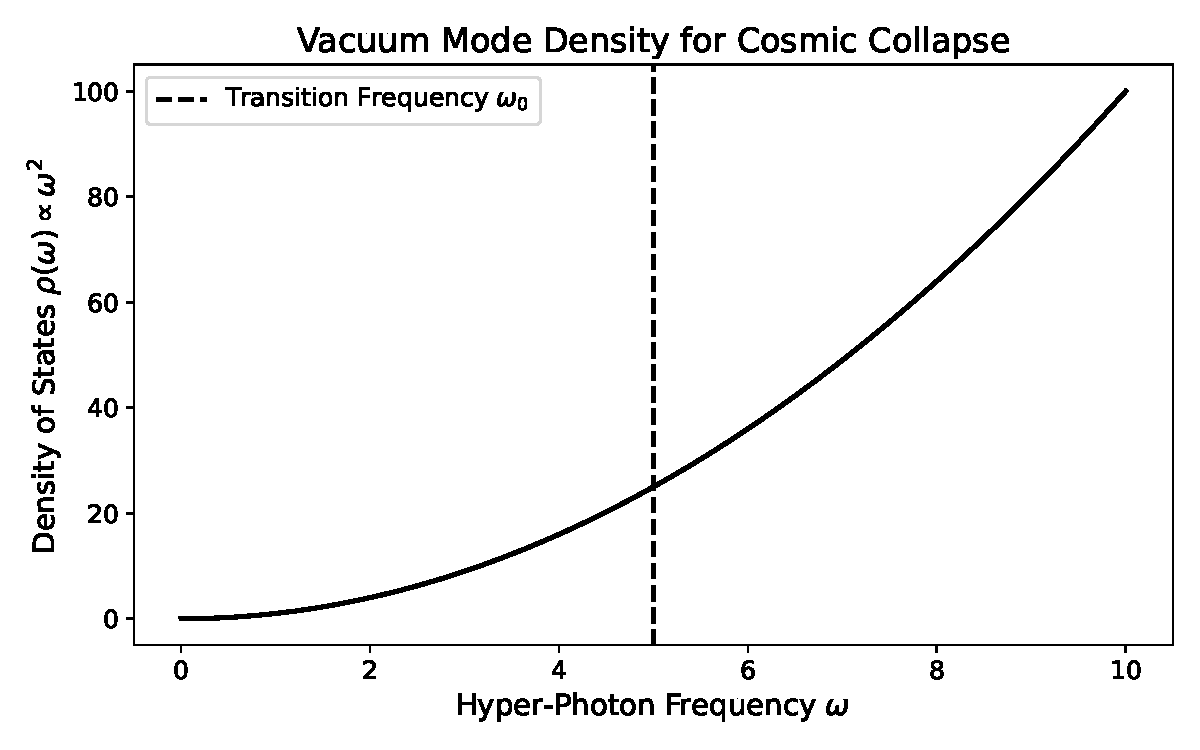
\includegraphics[width=0.85\textwidth]{fig_ch4.pdf}
\caption{Mathematical visualization of the principles derived in Section 4.}
\end{figure}
